\chapter{Methodology}
\vspace{-1.5cm}
\hspace{-1cm}\rule{19cm}{0.4pt} 

\section{Project Overview}
This project aims to create an automated system that can generate, test, and document scientific ideas with minimal human intervention on repetitive research tasks, without compromising rigor and quality. The methodology covers the whole pipeline of research, which has been divided into five major stages: idea generation, experimental design, data collection, analysis, and documentation.\\
It first creates the potential research ideas with input parameters or a predefined starting template, then it evaluates those ideas as to whether they are new and feasible using external sources such as academic databases, after which it designs the experiments for testing the remaining concepts. It does this through the development of a complete experimental setup that provides all the details on the method by which data will be gathered and analyzed.
\begin{figure}
    \centering
    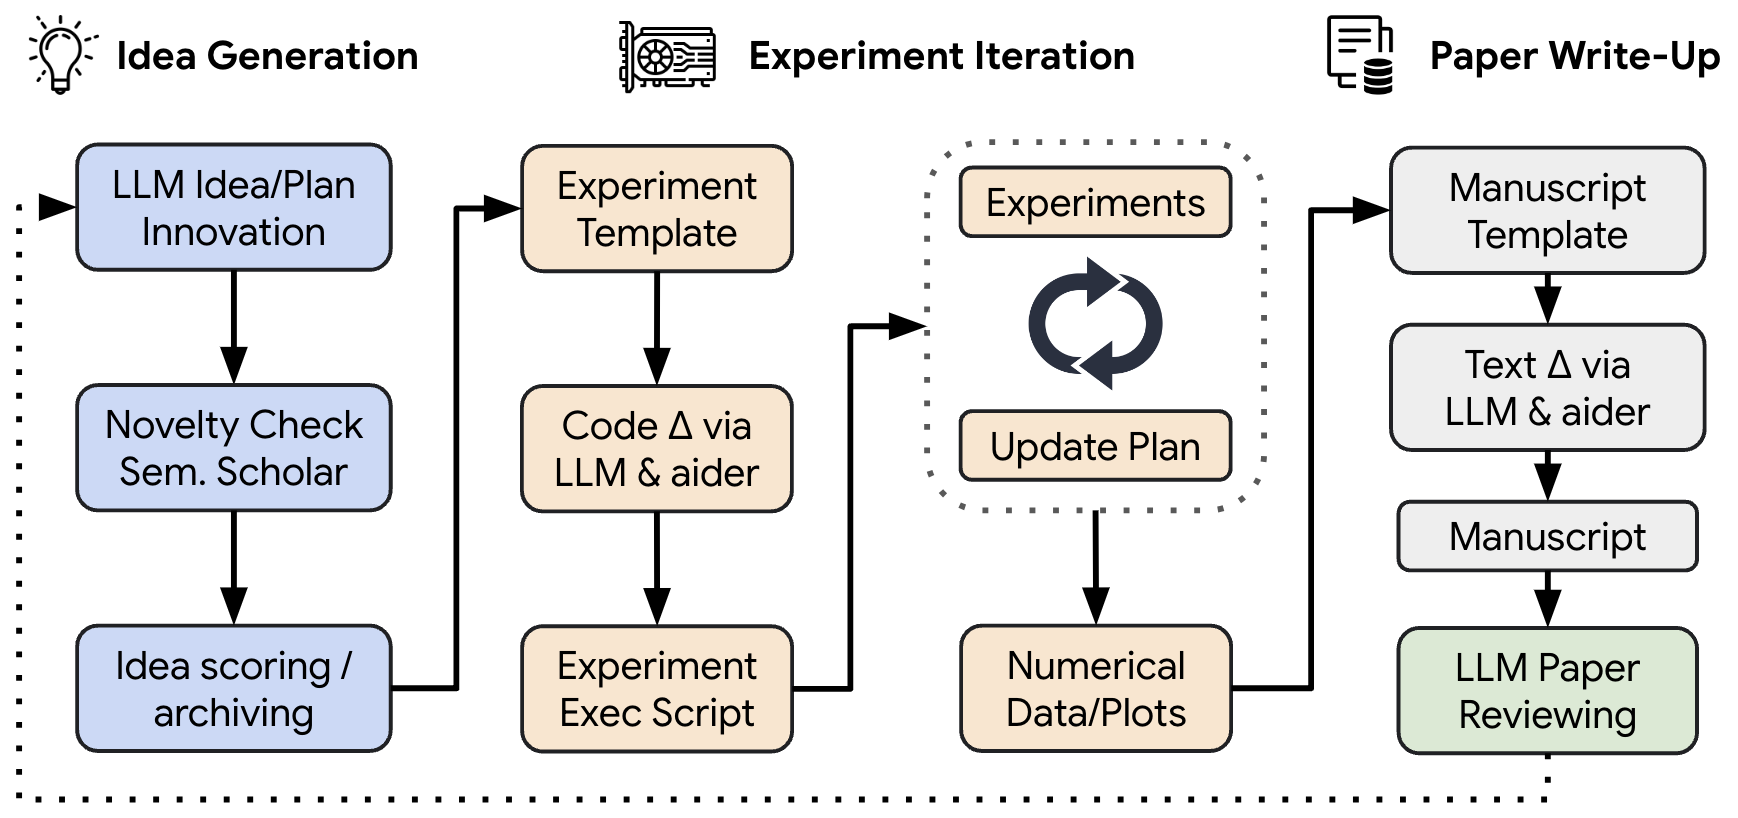
\includegraphics[width=0.8\textwidth]{images/flowchart.png}
    \caption{Overview of the automated research pipeline showing the main stages from ideation to documentation.}
    \label{fig:methodology} % chktex 24
\end{figure}

The experiments are therefore designed, conducted, and their data collected in an organized and systematic manner. At this level, the most important goal is to achieve reliable as well as relevant results against the hypotheses proposed. Consequently, the obtained data is analysed by using relevant statistical means and the outcomes are therefore presented in a structured reporting format that abides by conventional standards of professional academic work. This documentation includes interpretations of the findings, discussions on their implications, and suggestions for future research. To measure the success of the project, a combination of quantitative metrics, such as novelty scores and reproducibility rates, and qualitative reviews will be used. This includes simulated peer reviews, providing an understanding of how well the automated system produces valuable research outputs and whether it complies with scientific standards. \\
The project will be initially tested within a computational domain to ensure practicality and effectiveness. Following this phase, the system's adaptability for broader fields of research will be evaluated, assessing its potential application in various scientific disciplines beyond its original scope.

\section{Research Design and Approach}
The research design for this project is set as an iterative, modular process with feedback loops to enable continuous improvement. The dominant approach follows a number of key stages that are important to the overall functionality of the automated system:
\begin{enumerate}
    \item \textbf{Idea Generation}
    \begin{itemize}
        \item \textbf{Diverse Hypothesis Generation:} Through computational models, the system creates a diverse set of hypotheses or research questions. This is done through randomization and guided generation based on existing knowledge within a scope.
        \item \textbf{Novelty Assessment:} Tools such as semantic search APIs are integrated to assess the novelty of ideas generated, ensuring that the ideas are novel and do not duplicate work already done.
    \end{itemize}

    \item \textbf{Experimental Design}
    \begin{itemize}
        \item \textbf{Testable Hypotheses:} Every formed hypothesis is turned into a testable hypothesis and then used for designing experiments according to specific domain needs.
        \item \textbf{Reusable Code Templates:} Code template libraries are modified so the system can dynamically change experiment designs in response to user feed back from preliminary testing rounds. This improves versatility and reactivity.
    \end{itemize}

    \item \textbf{Data Gathering}
    \begin{itemize}
        \item \textbf{Implementation of Experiments:} Conducting the experiment on preselected sets or simulated scenarios generates measurable data.
        \item \textbf{Automation for Robustness:} Multiples of the experiments are run using automation to establish robustness and reliability of the results.
    \end{itemize}

    \item \textbf{Analysis and Documentation}
    \begin{itemize}
        \item \textbf{Statistical Analysis:} Results will be analyzed through statistical tools or machine learning pre-programmed to help determine the patterns and insights that come out.
        \item \textbf{Structured Documentation:} The findings are presented in an academic manner using visualizations and structured text according to professional research reporting standards.
    \end{itemize}

    \item \textbf{Evaluation}
    \begin{itemize}
        \item \textbf{Automated Review Mechanism:} An automated review mechanism evaluates the clarity, originality, and potential impact of the documented work, simulating a peer-review process. This provides valuable feedback on the quality of the research outputs.
    \end{itemize}
\end{enumerate}

\section{Data Collection Methods}
Data Collection Methods
Data collection in this project is fully automated, using pre-existing datasets, simulated environments, and self-generated experimental results. The methods used in this process include:
\begin{enumerate}
    \item \textbf{Predefined Datasets}\\
    Integration of Relevant Datasets: Datasets that are pertinent to the research domain are identified and integrated into the experimental setup. These datasets may be either publicly available or generated by the system itself, depending on the specific scope of the project.

    \item \textbf{Simulated Experiments}\\
    Usage of Simulated Data Environments: Whenever real-world data is unavailable or infeasible to be collected, the system relies on simulated data environments. This way, it achieves flexibility and scalability and allows one to experiment without the confinements of real-world data.

    \item \textbf{Real-Time Data Logging}\\
    All relevant data during experimental runs, including intermediate results, errors, and performance metrics, are recorded by the system. These logs are systematically saved for later analysis, providing a detailed record of how each experiment was executed.

    \item \textbf{Dynamic Data Collection}\\
    Modification of Experimental Parameters: The system is designed to modify experimental parameters during the run, thus allowing data collection under different conditions. This capability ensures that results are comprehensive and reliable by capturing a wide range of outcomes based on different experimental settings.
\end{enumerate}

\section{Data Analysis Techniques}
This process of data analysis for the project aims at deriving meaningful insights with a high validity and reproducibility of the results. The most basic statistical methods such as mean, standard deviation, and confidence intervals are used to summarize and assess the outcomes of experiments. It is basically an easy foundational analysis of understanding central tendencies and variability.
Comparison of the results from different experimental setups is used to assess the efficiency of various approaches. Comparative analysis includes evaluation against the baseline results or established benchmarks, which can provide an understanding of how different methodologies perform relative to one another.
Data visualizations are crucial in the analytical process. The system develops plots, graphs, and heatmaps to depict trends, relationships, and anomalies in data. Libraries like Matplotlib or Seaborn are often used to create them in Python and enhance the interpretability of the results.\\
Error and failure analysis is also performed when experiments do not deliver expected results. In such cases, potential flaws in design or execution can be pinpointed. It's a crucial feedback loop in ensuring that the research process stays adaptive and responsive for the improvements of the following iterations.\\
Finally, to avoid losing clarity and academic value in the presentation of findings, the system uses natural language generation techniques for summarization. This ensures findings are communicated effectively, but they are also accessible to a wider audience while holding scholarly standards. Overall, this comprehensive data analysis process supports the goal of producing high-quality research outputs by the project.

\section{Ethical Considerations}
This project recognizes the ethical concerns of automating scientific research and follows principles intended to mitigate risks and encourage responsible use. One of the key concerns is transparency: all outputs generated by automation, such as research results and reviews, are appropriately labeled as system-generated in order to maintain accountability. Transparency is essential to preserve trust in the research process.\\
Another key emphasis is on the mitigation of bias. Proactive efforts in the form of mitigation are made regarding biases generated while coming up with ideas, while selecting the data and when interpreting results by using varied datasets and strict evaluation criteria to enhance objectivity from research outputs.
Another area of concern is related to data privacy. When one uses external datasets, the project ensures compliance with data protection laws and ethical guidelines when not collecting or analyzing sensitive data or personal data. So, in such a regard, data privacy protects and respects individual rights and complies with the ethical and moral code in research practice. Safeguards are provided for the system to not create unethical or harmful research ideas. A review mechanism exists that flags potentially problematic outputs so that timely intervention and correction can be undertaken.\\
Responsible deployment is a guiding principle of this project. The system is designed to assist and complement human researchers, not replace them. The outputs are designed to inspire and guide further exploration, not definitive conclusions. Through the emphasis on collaboration between automated systems and human expertise, the project promotes a responsible and ethical approach to scientific inquiry.

\section{Limitations}
While the project demonstrates significant advancements in automating research workflows, it is not without limitations. These challenges must be acknowledged to ensure a realistic understanding of the system's capabilities and areas for improvement.
\begin{enumerate}
    \item \textbf{Domain Dependency}\\
    The effectiveness of the system is highly dependent on the availability of structured datasets and domain-specific knowledge. Certain fields may require additional customization to ensure that the outputs generated are meaningful and relevant. This dependency can limit the system's applicability across diverse research areas, necessitating tailored approaches for different domains.

    \item \textbf{Computational Constraints}\\
    Running experiments, particularly those involving large datasets or complex simulations, can be resource-intensive and costly. The computational demands may pose challenges for users with limited access to high-performance computing resources, potentially restricting the system's widespread adoption.

    \item \textbf{Error Propagation}\\
    Errors that occur in one stage of the research pipeline—such as experiment design—can propagate to subsequent stages, potentially compromising the final output. This risk highlights the importance of rigorous validation and quality control measures throughout the entire process to minimize the impact of errors.

    \item \textbf{Limited Context Understanding}\\
    Although the system is designed to generate results and reports, it lacks the nuanced understanding that a human researcher possesses. This limitation may result in overly simplistic interpretations of complex findings, underscoring the need for human oversight in interpreting results and drawing conclusions.

    \item \textbf{Ethical and Safety Concerns}\\
    There is an inherent risk of misuse, such as generating low-quality or misleading research outputs. Ensuring oversight and regulation is critical to mitigate these risks and uphold ethical standards in research. Continuous monitoring and evaluation mechanisms will be necessary to address potential ethical concerns associated with automated research generation.
\end{enumerate} 